\section{Описание разработанной системы}

В данной главе будет рассмотрена общая архитектура фаззера, описан процесс конфигурации и использования фаззера конечным пользователем.

\subsection{Общая архитектура}

Разработанную систему можно условно поделить на компоненты, которые также приведены на рисунке \ref{fig:arch} далее:
\begin{itemize}
	\item библиотека образцов, ответственная за хранение состояния фаззера и выбор очередного кандидата на мутацию на основании хранимой информации о покрытии, как было описано выше;
	
	\item подсистема, ответственная за генерацию данных, выполняющая мутацию и кроссинговер для выбранного ранее образца на базе имеющейся библиотеки. Данный компонент постепенно изменяет параметры распределения вероятностей выбора из имеющихся мутаторов в соответствии с полученными данными о покрытии;
	
	\item подсистема, осуществляющая запуск исполняемого файла. При запуске через файл или стандартный ввод (в зависимости от конфигурации) передаётся очередной образец, выполняется трассировка исполняемого файла при помощи ptrace, как было описано ранее, и в результате мы получаем данные о покрытии (Trace);
	
	\item подсистема, ответственная за вывод информации на экран. Пользователю предоставляется информация о том, как протекает процесс тестирования для информирования и возможной диагностики неполадок.

\begin{figure}[h]
	\centering
	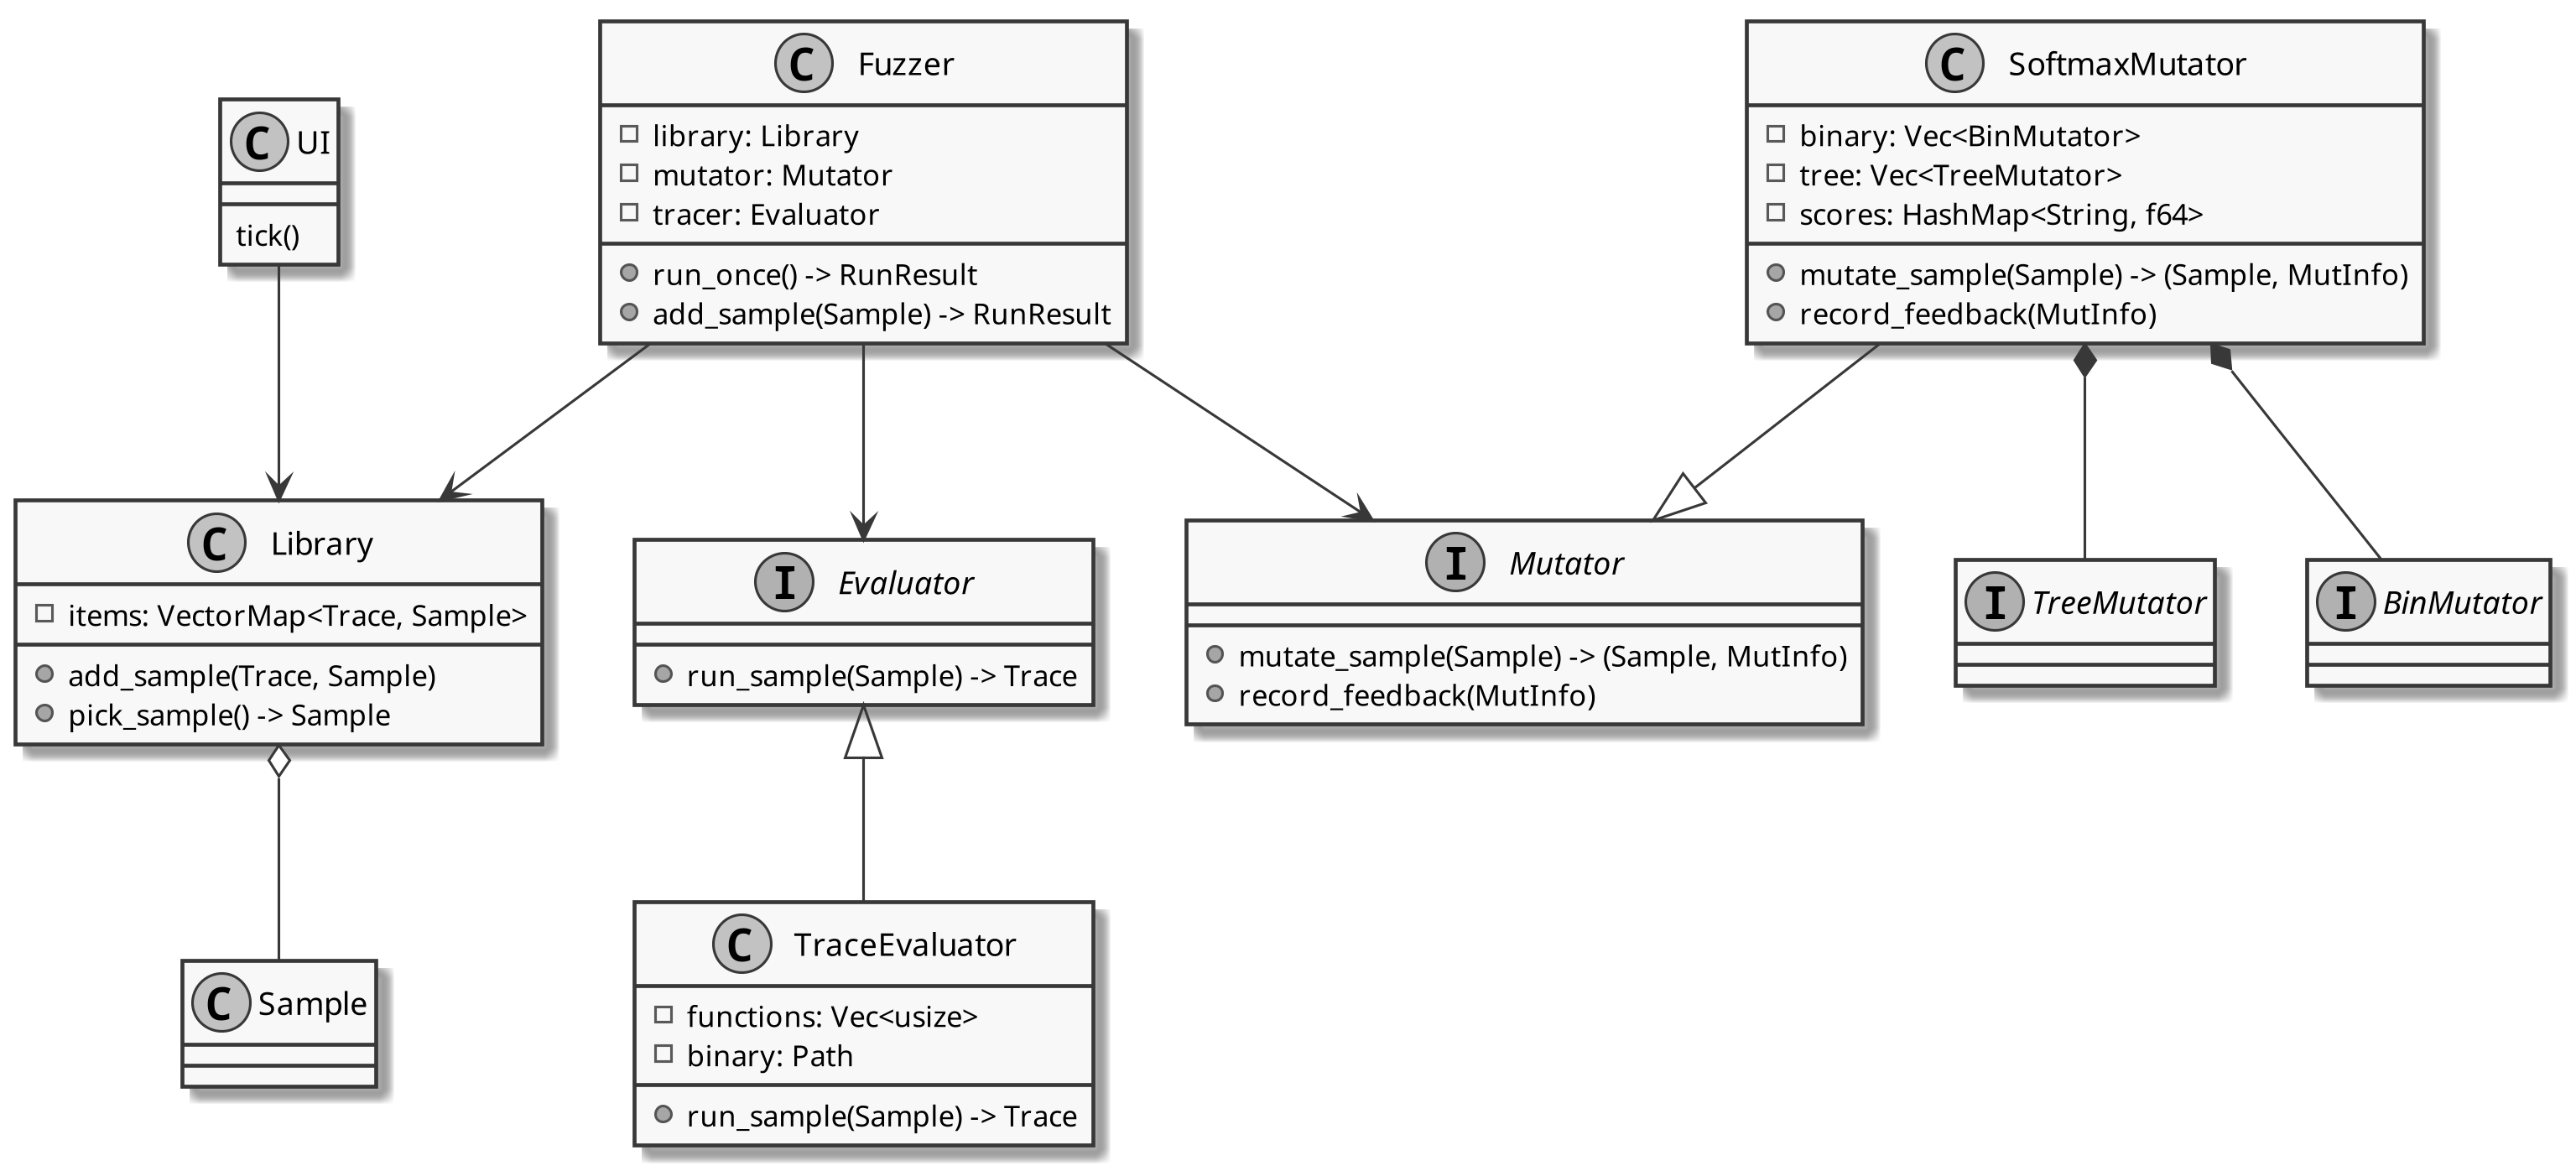
\includegraphics[width=0.99\textwidth]{arch.png}
	\caption{Диаграмма классов системы}
	\label{fig:arch}
\end{figure}%
	
\end{itemize}

В качестве языка реализации был использован язык системного программирования Rust \cite{rust}, поскольку он предоставляет доступ ко всем необходимым системным вызовам и интерфейсам операционной системы и в то же время обладает субъективно высоким уровнем удобства.

\subsection{Конфигурирование}

Для конфигурирования фаззера используется формат Toml. В едином файле fuzz.toml пользователь указывает исполняемый файл, который хочет тестировать, описывает, что будет подаваться на вход, а также при необходимости указывает дополнительные данные, например параметры для алгоритма выбора методов мутации или параметры отдельных мутаторов. Простейшая конфигурация выглядит следующим образом:

\begin{code}
[binary]
# путь до исполняемого файла
path = "./exif"
# указание, как данные будут подаваться на вход
# (stdin по-умолчанию)
pass_style = "file"

[input]
# папка с образцами
seeds = "./examples"
\end{code}

Система допускает задание входа либо в виде готовых примеров и в таком случае будет использовать исключительно бинарные мутации, как это делают классические фаззеры, либо в виде грамматики, и в таком случае пользователю дополнительно нужно будет описать вход в отдельном файле в виде контекстно-свободной грамматики. Грамматика задаётся набором алтернативных продукций вида \ic{N -> P\_1|...|P\_N}, где \ic{N} это нетерминал, а \ic{P\_i} -- один или более элемент из следующего набора:

\begin{itemize}
	\item другой нетерминал, записывающийся по привычному для языков программированиям правилам: первый символ является буквой или символом подчёркивания, а последующие буквами, цифрами или символами подчёркивания (например, \ic{root} или \ic{Number});
	
	\item фиксированная строка, ограниченная двойными кавычками (например, \ic{"SELECT"}). Данный элемент оказывается полезным для описания грамматик, порождающих текстовый ввод;
	
	\item строка, задаваемая регулярным выражением. Для задания регулярного выражения обычную строку следует заключить в re(...), например \ic{re("[a-z][a-z]+")}. Стоит отметить, что функционал регулярных выражений можно эмулировать и с помощью продукций, данный функционал введён для повышения удобства;
	
	\item фиксированная последовательность байт, задаваемая в шестнадцатиричном виде с префиксом 0x, например \ic{0x89504e47}. Данный тип токенов может быть полезен при описании бинарных форматов файлов, например для задания магических чисел -- приведённый ранее пример является magic для файлов формата png;
	
	\item произвольный набор байт, задаваемый литералом bytes. Позволяет указать либо сегмент фиксированной длины (например \ic{bytes(4)}) либо сегмент с длиной в некотором диапазоне (\ic{bytes(5 8)});
	
	\item специальный токен Nothing, позволяющий указывать пустые продукции (это полезно для записи опциональных секций через правило вида \ic{Marker -> 0x9F | Nothing}).
\end{itemize}

Пример грамматики, составленной по данным правилам:
\begin{code}
root -> "SELECT " select_target " FROM " name;
select_target -> "*" | args;
args -> name | args ", " name;
name -> re("[a-z][a-z0-9]*");
\end{code}

\subsection{Пользовательский интерфейс}

Для наблюдения за процессом тестирования и диагностики возможных ошибок конфигурации пользователю предоставляется простой интерфейс в виде терминальной превдографики, который можно видеть на рисунке \ref{fig:tui} ниже. В нём можно выделить четыре секции:

\begin{enumerate}
	\item информация о времени тестирования, сообщающая пользователю о том, как долго протекает процесс тестирования и как давно происходили некоторые интересные события (обнаружение новых путей в программе и обнаружение уникальных крашей);
	
	\item информация о запуске программы, отображающая общее число запусков и разбивку по категориям (успешное завершение, с кодом ошибки, краш), а также среднюю скорость выполнения и число успешных минимизаций тестовых примеров;
	
	\item информация о том, как много уникальных поведений программы -- путей, кодов возврата и крашей -- было обнаружено;
	
	\item секция с сообщениями системы.
\end{enumerate}

\begin{figure}[h]
	\centering
	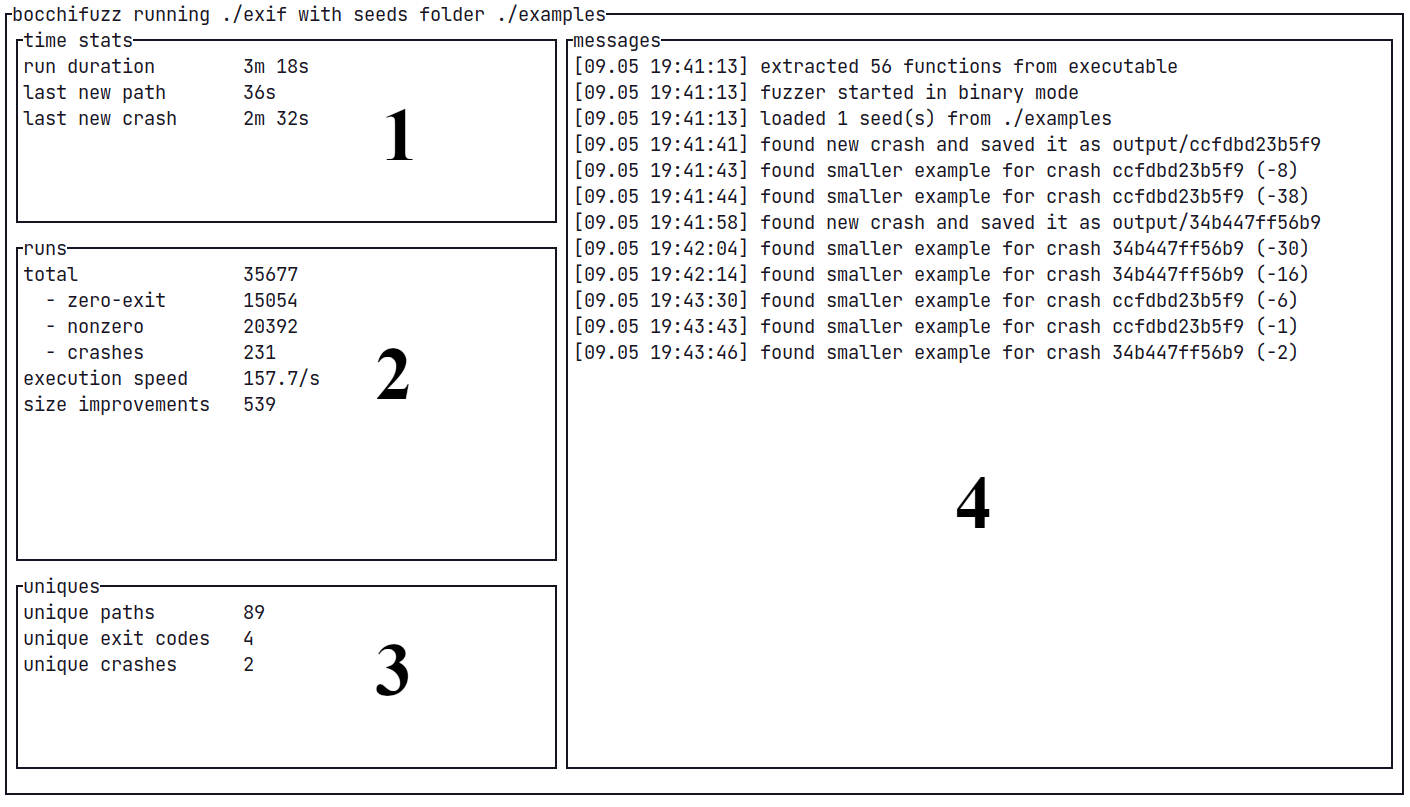
\includegraphics[width=0.99\textwidth]{tui.png}
	\caption{Терминальный интерфейс}
	\label{fig:tui}
\end{figure}%

\subsection{Экспорт результатов тестирования}

Простого применения фаззера как правило оказывается недостаточно для локализации источника или построения эксплойта на основе обнаруженной уязвимости. Исследователь, вероятно, захочет воспользоваться дебаггером для анализа поведения программы на обнаруженном примере или запустить систему для автоматической генерации ROP-цепочки. По этой причине стоит озаботиться экспортом результатов тестирования в удобном для дальнейшей обработки программными средствами формате.

Основным результатом работы фаззера является набор тестовых примеров, приводящих к падению программы. Образцы, получаемые по мере работы системы, сохраняются в настраиваемую пользователем директорию под уникальными именами, после чего их можно с лёгкостью подать на вход программе средствами командной оболочки либо же загрузить встроенными средствами применяемого языка программирования. В случае, если пользователю нужна дополнительная информация о конкретном примере, таковую можно получить из соответствующего события в журнале.

Формат JavaScript Object Notation (далее -- JSON) является распространённым форматом обмена данными в клиент-серверных приложениях, в связи с чем инструментарий для работы с JSON присутствует по-умолчанию во многих современных языках программирования, что делает его привлекательным форматом для сериализации данных. События, возникающие в процессе фаззинга (например, обнаружение нового пути) сохраняются в виде newline-delimited JSON (далее -- NDJSON), то есть отдельные записи в файле представляют из себя JSON-объекты, которые отделяются друг от друга переводом строки. Таким образом сохраняется информация о времени возникновения того или иного события, его типе и других ассоциированных с ним данных.